\subsection{Environment}

\begin{figure}
    \centering
    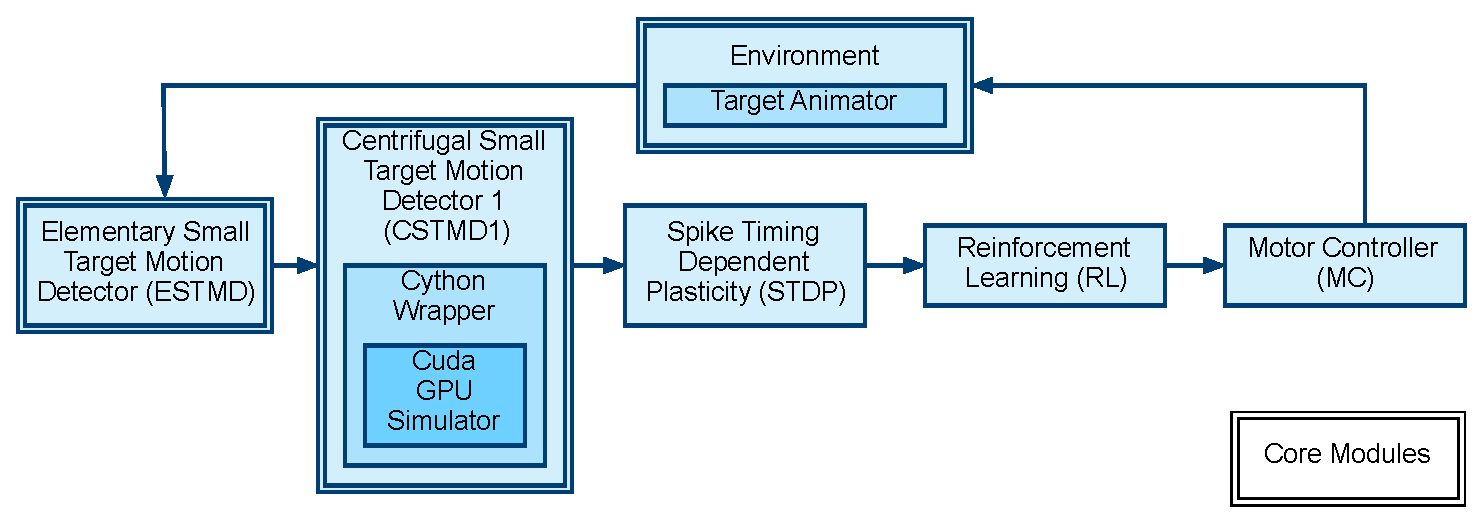
\includegraphics[width = 0.7\textwidth]{Figures/Project_Structure_Revised-2.eps}
    \caption{Project Structure}
    \label{fig:structure}
\end{figure}

The environment builds upon the \textit{Target Animation} module developed by the previous group \cite{GITHUB1}. The code has been refactored and extended to abstract the animation process away from the environment state (e.g the dragonfly velocity). However it still enables the animation of the dragonfly's prey (targets, represented by black dots) that either move randomly around a fixed point or with a constant velocity.

Many of the functions have been rewritten to increase efficiency and to suit the holistic integrated design. This includes the addition of a step function that updates the dragonfly's and preys' positions given a specified velocity (from the Motor module) and outputs an array at each time-step. This will be a more efficient input to the ESTMD module compared with the encoding and subsequent decoding of a video file, which was done before.

Due to the need for graphics dependencies we have wrapped a working version of \textit{Target Animation} as a Docker image, allowing it to be run with all dependencies pre-installed.